\chapter{Index Analysis of the MNA}

der ane satz do + proof hopefully

seite 22 kap 7 netw top and dae ind for rlc - modelling and discretization circ prob

In the linear case, the capacitances, inductances and resistances are symmetrical positive definite (We consider them as matrices in this case). In the nonlinear case ... . Then it is called an RLC network.

In our further analysis we will only consider such RLC networks.

This means we consider the equations resulting from the analysis above. As a reminder, these equations are of the form \ref{DAE-const-coeff}

\begin{displaymath}
	A y'(t) + B y(t) = f(t).
\end{displaymath}

Specifically the obtained equations from the Modified Nodal Analysis \ref{MNA_Matrixform} are

\begin{displaymath}
	\begin{pmatrix}
		A_C C A_C^\top & 0 & 0 \\
		0 & L & 0 \\
		0 & 0 & 0
	\end{pmatrix}
	*
	\begin{pmatrix}
		\dot{u} \\
		\dot{i_L} \\
		\dot{i_V}
	\end{pmatrix}
	+
	\begin{pmatrix}
		A_R G A_R^\top & A_L & A_V \\
		-A_L^\top & 0 & 0 \\
		-A_V^\top & 0 & 0 ä
	\end{pmatrix}
	*
	\begin{pmatrix}
		u \\
		i_L \\
		i_V
	\end{pmatrix}
	=
	\begin{pmatrix}
		-A_I i_{src} \\
		0 \\
		-v_{src}
	\end{pmatrix}
\end{displaymath}

\section{General Index analysis}

Assuming the system only contains linear elements or is linearized at an operating point in order to investigate the system behaviour then the corresponding network equation represent a DAE with constant coefficients \ref{DAE-const-coeff}. We will denote $x=(u i_L i_V)^\top$.

\begin{itemize}
	\item \textbf{ODE-case}: \newline
	The matrix $B$ is regular in \ref{DAE-const-coeff}. This is the case if
	\begin{figure}[H]
		\centering
		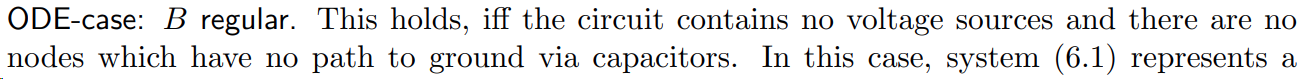
\includegraphics[width=0.7\linewidth]{screenshot006}
		\caption{}
		\label{fig:screenshot006}
	\end{figure}
	, then the system represents  a linear-implicit system of ODEs and can be transformed into the explicit ODE sytstem.
		
	\item \textbf{DAE-case}:
	The matrix $B$ is singular in \ref{DAE-const-coeff}. In the following we will assume $D$ to be regular. Multiplying with $D^{-1}$ from the left side produces
	\newline
	nevermind thats the same as we did in the \ref{DAE-const-coeff} chapter. - reference to that an explain in these terms. - page 20
\end{itemize}

The index of the MNA is the same as $ind(A,B)$, which denotes the nilpotency index of $N$ as we have seen in the previous analysis in chapter 3.


Investigating the index-cases further we can again distinct into two cases:

reminder for the structure obtained in previous chapter
\begin{align*}
	u'(t) + Ru(t) &= s(t), \\
	Nv'(t) + v(t) &= q(t)
\end{align*}

\begin{enumerate}
	\item index 1 case
	Because $N$ is nilpotent with nipotency index $\nu = 1$ it holds that $N^1 = 0$, thus the system transforms to
	\begin{align*}
		u'(t) + Ru(t) &= s(t), \\
		v(t) &= q(t).
	\end{align*}
	This means that the algebraic variables are given explicitly. Thus the system can be written in ODE form
	\begin{displaymath}
		\dot{x}=B^{-1}(-Ax+f(t)).
	\end{displaymath}

	\item index $\geq$ 2 case
	
	results in the solution we derived in \ref{solution-to-transformed-DAE-const-coeff-part2}.
\end{enumerate}

continue herer with modelling book from bottom of page 20-21

\section{Topological Conditions}
For this we consider RLC networks with independant voltage and current sources (\textbf{what does that mean?}). To obtain the perturbation index of the MNA we perturb the right-hand side of  
\newline reference to Tischendorf

basically chapter 7 of modelling book

From analyzing the MNA some conditions to the circuit topology can be obtained. We will be concidering the impact of loops containing only capacitances and voltage sources as well as cutsets containing only inductances and current sources.

\begin{theorem}[Index-1 condition] \cite{Tischendorf2004Topological}
	Let the matrices of the capacitances, inductances and resistances respectively be positive definite. If the network neither cointains \emph{inductance-current-source cutsets} nor (controlled?) \emph{capacitance-voltage-source loops}, then the MNA leads to an index-1 DAE.
\end{theorem}

\begin{theorem}[Index-2 condition] \cite{Tischendorf2004Topological}
	If the Network contains \emph{inductance-current-source cutsets} or \emph{capacitance-voltage-source loops} except for capacitance-only loops, then the MNA leads to an index-2 DAE.
\end{theorem}